\chapter{Brudgrænsetilstand}

I dette afsnit undersøges tilbygningens brudgrænsetilstand. Først beregnes reaktionerne ud fra Figur \ref{fig:alle} og dernæst laves snitkræfter. Slutteligt undersøges spændingstilstanden, og udfra ståltypens flydespændingen kan det vurderes, om konstruktionen kan holde eller vil bryde sammen.   

\section{Reaktioner}
Reaktionerne i de tre understøtninger beregnes ved at opdele konstruktionen. Systemet opdeles i det midterste charnierled i henholdvis en venstre- og højre del, som ses på Figur \ref{fig:opdelingv} og \ref{fig:opdelingh}. I skæringen mellem de to dele, vil der være snitkræfter, men ikke momentkræfter, da momentet i charnierledet er nul. Dermed optræder der kun normalkraften, N, og forskydningskraften, V.

\begin{figure}[H]
	\centering
	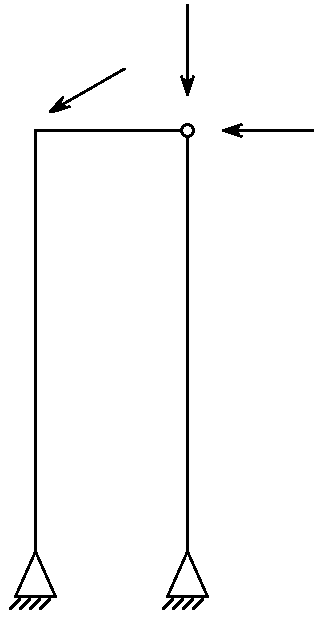
\includegraphics[width=0.7\textwidth]{billeder/venstre.png}
	\caption{Venstre side af systemet med reaktioner, samt fritlegemediagram}
	\label{fig:opdelingv}
\end{figure}

\begin{figure}[H]
	\centering
	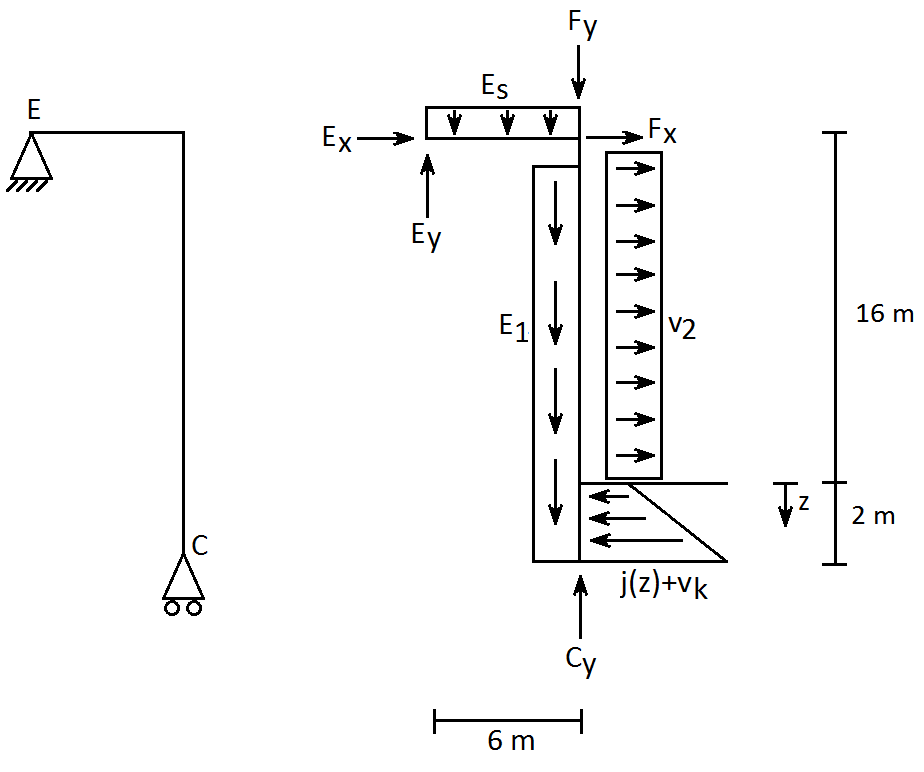
\includegraphics[width=0.7\textwidth]{billeder/hojre.png}
	\caption{Højre side af systemet, samt fritlegemediagram}
	\label{fig:opdelingh}
\end{figure}

Reaktionerne på højre side af systemet, der virker i charnieret, sættes som belastninger på venstre del af systemet. Reaktionerne på højre del af systemet beregnes først.
\newline
\newline
Først bestemmes den vandrette reaktion i charnier ledet, $S_v$ gennem vandret ligevægt: 
\begin{center}
	$\rightarrow+:0 = F_x + E_x - J(2m) - V_k \cdot 2m - V_2 \cdot 16m$
	\newline
	$E_x = -1,\!45 kN$
\end{center}

$C_y$ bestemmes gennem moment ligevægt om punkt E: 
\begin{center}
	$\AR{}:0 = -F_y \cdot 6m - E_1 \cdot 18m \cdot 6m + C_y \cdot 6m - J(2m) \cdot 17,\!33m - V_k \cdot 2m \cdot 17m - E_s \cdot 6m \cdot 3m - V_2 \cdot 16m \cdot 8m$
	\newline
	$C_y = 779,\!83 kN$
\end{center}

Til sidst bestemmes den lodrette reaktion i charnier ledet, $S_l$ gennem lodret ligevægt: 
\begin{center}
	$\uparrow+: 0 = F_y - E_1 \cdot 18m - E_s \cdot 6m + C_y + S_l$
	\newline	
	$E_y = -164,\!89 kN$
\end{center}

Reaktionerne $E_y$ og $E_x$ påsættes som belastninger i punkt E på det venstre system. Da reaktionerne i begge systemer peger i negativ retning, ændres fortegnet og dermed retning, så de virker som vist på Figur \ref{fig:opdelingv}.
\newline \indent{     } Reaktionerne i det venstre system kan hermed bestemmes.
\newline
\newline
Først tages der moment om A, for at beregne $B_y$  
\begin{center}
	$A\hookrightarrow+: 0 = B_y \cdot 6m + E_y \cdot 6m + E_x \cdot 18m - E_2 \cdot 18m \cdot 6m - E_s \cdot 6m \cdot 3m + D_x \cdot 18m - V_1 \cdot 16m \cdot (8m + 2m) - J(2m) \cdot (2m \cdot \frac{1}{3}) - V_k \cdot 2m \cdot 1m$
	\newline 
	$B_y = 127,\!92 kN$
\end{center}

Nu laves lodret ligevægt for at bestemme $A_y$
\begin{center}
	$\uparrow+: 0 = A_y + B_y - E_y - E_2 \cdot 18m - E_1 \cdot 18m - F_y - E_s \cdot 6 m$
	\newline
	$A_y = 547,\!96 kN$
\end{center}

For at gøre det muligt at isolere en af de vandrette reaktioner laves der et snit i charnieret, og derefter tages der moment omkring charnieret i punkt E, for at bestemme $B_x$:
\begin{center}
	$\hookrightarrow+: 0 = B_x \cdot 18m$
	\newline
	$B_x = 0 kN$
\end{center}

Slutteligt laves vandret ligevægt for at bestemme $A_x$
\begin{center}
	$\rightarrow+: 0 = A_x - E_x + B_x + J(2m) + V_k \cdot 2m + V_1 \cdot 16 m - D_x$
	\newline
	$A_x = -133,\!31 kN$
\end{center} 

\section{Snitkræfter}
Snitkræfterne for tilbygningen Strøybergs Palæs stålramme kan nu beregnes. Her laves der syv snit, som er illustreret på Figur \ref{fig:snitbrud}. Disse resultater vil bruges til at undersøge, om konstruktionen har en tilstrækkelig bæreevne eller om den vil bryde sammen. 

\begin{figure}[H]
	\centering
	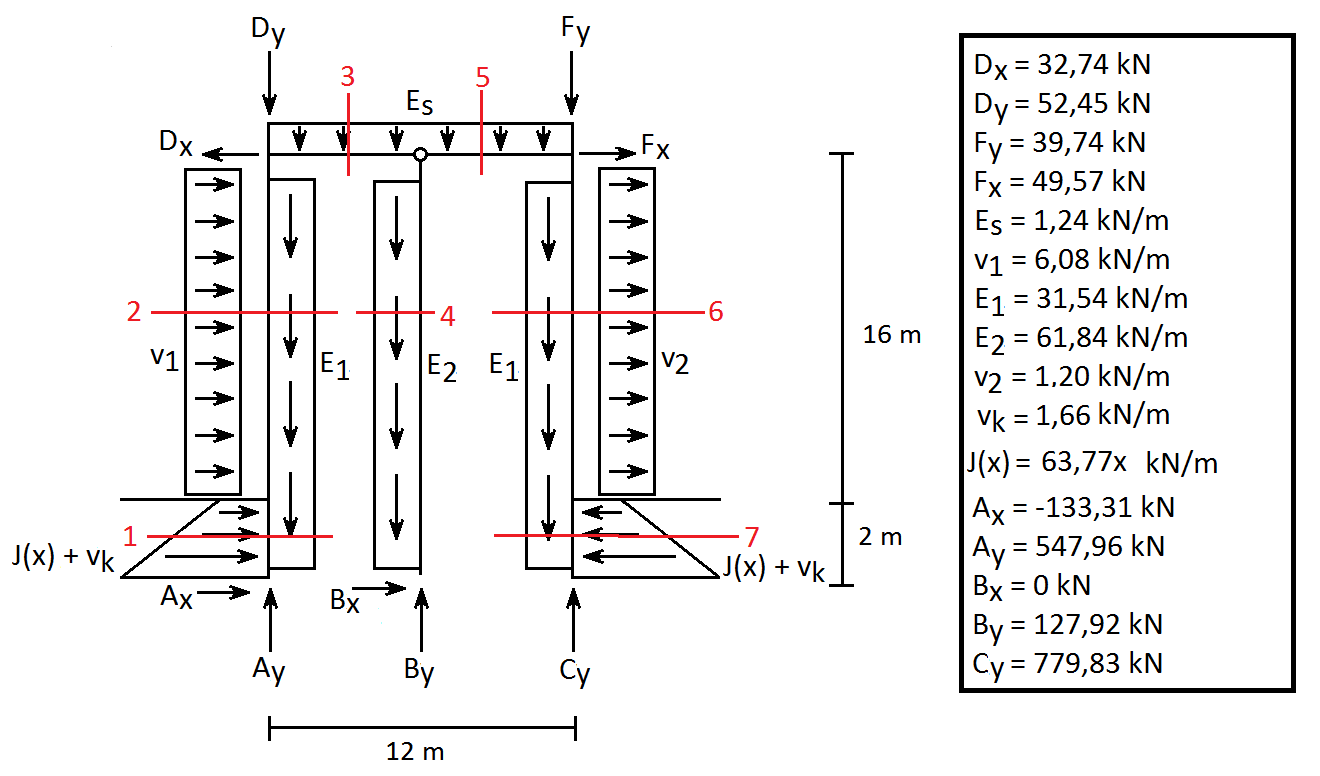
\includegraphics[width=0.8\textwidth]{billeder/snitbrud.png}
	\caption{Snit}
	\label{fig:snitbrud}
\end{figure}

Nedenfor vises beregningseksempel for snit 1 og snit 5. Beregningerne for de resterende snit, kan ses i Bilag ???. 
\newline
\newline
\textbf{Snit 1: 0 < x < 2 m}
\newline
Fritlegemediagrammet for snit 1 ses på Figur ???.
\newline
\newline
Først bestemmes normalkraften:
\begin{center}
	$0 = N_1 + A_y - E_1 \cdot x \leftrightarrow N_1(x) = 31,\!54 \frac{kN}{m} x - 547,\!95 kN $
\end{center}

Normalkraften bestemmes ved 0 m og 2 m:
\begin{center}
	$N_1(0m) = -547,\!95 kN$
	\newline
	$N_1(2m) = -484,\!87 kN$
\end{center}

Nu bestemmes forskydningskraften:
\begin{center}
	$0 = V_1 + J(x) + v_k \cdot x + A_x \leftrightarrow V_1(x) = -33,\!64\frac{kN}{m} x + 133,\!31 kN$
\end{center}

Forskydningskraften bestemmes ved 0 m og 2 m:
\begin{center}
	$V_1(0m) = 133,\!31 kN$
	\newline
	$V_1(2m) = 66,\!02 kN$
\end{center}

Til sidst bestemmes momentkraften:
\begin{center}
	$0 = M_1 + J(x) \cdot \frac{2x}{3} + v_k \cdot x \cdot \frac{x}{2} + A_x \cdot x \leftrightarrow M_1(x) = -22,\!15\frac{kN}{m} x^2 + 133,\!30kN x$
\end{center}

Momentkraften i højden 0 m og 2 m bestemmes:
\begin{center}
	$M_1(0m) = 0 kNm$
	\newline
	$M_1(2m) = 178,\!00 kNm$
\end{center}

\textbf{Snit 5: 0 < x < 6 m}
\newline
\newline
Normalkraften bestemmes først:
\begin{center}
	$0 = -N_5 + F_x - v_2 \cdot 16m - J(2m) - v_k \cdot 2m \leftrightarrow N_5 = 49,\!57 kN - 48,\!12 kN = 1,\!45 kN$
\end{center}

Hermed er normalkraften til 0 m og 6 m 1,45 kN. 
\newline
\newline
Forskydningskraften for snit 5 bestemmes ved:
\begin{center}
	$0 = V_5 - E_1 \cdot 18 m - F_y + C_y - E_s x \leftrightarrow V_5(x) = -172,\!35 kN + 1,\!24 \frac{kN}{m}x$
\end{center}

Forskydningskraften til 0 m og 6 m er hermed:
\begin{center}
	$V_5(0m) = -172,\!35 kN$
	\newline
	$V_5(6m) = -164,\!89 kN$
\end{center}

Til sidst bestemmes momentkraften:
\begin{center}
	$0 = -M_5 - F_y \cdot x - E_1 \cdot 18 m \cdot x - E_s \cdot x \frac{x}{2} - v_2 \cdot 16 m \cdot 8 m - v_k \cdot 2 m \cdot 17 m - J(2m) \cdot 17,\!33 m + C_y \cdot x \leftrightarrow M_5(x) = 172,\!35 kN \cdot x - 0,\!62 \frac{kN}{m} \cdot x^2 -1011,\!72 kNm$
\end{center}

Momentkraften til 0 m og 6 m bestemmes:
\begin{center}
	$M_5(0m) = -1011,\!72 kNm$
	\newline
	$M_5(6m) = 0 kN$
\end{center}


TABEL MED RESULTATER

\section{Spænding}
For at finde ud af om konstruktionen kan holde, undersøges spændingstilstanden. Her skal det gælde:

\begin{center}
	$\sqrt{\sigma^2 + 3\tau^2} \le f_y$ 
\end{center}

\begin{itemize}
	\item[-] $\sigma$: Normalspænding
	\item[-] $\tau$: Forskydningsspænding
	\item[-] $f_y$: Flydespænding
\end{itemize}

Flydespændingen beregnes ved formlen:

\begin{center}
	$f_y = \frac{f_{yk}}{\gamma}$
\end{center}

\begin{itemize}
	\item[-] $f_{yk}$: Den karakteristiske flydespænding, der afhænger af ståltype. For ståltype S235 er $f_{yk} = 225 MPa$
	\item[-] $\gamma$: Partialkoefficient, der sættes til 1,1 \citep[ s. 212]{stabi}.  
\end{itemize}

Altså beregnes den regningsmæssige flydespænding til:

\begin{center}
	$f_y = \frac{225 MPa}{1,\!1} = 204,\!54 MPa$
\end{center}

Normalspændingen findes ved Naviers formel:

\begin{center}
	$\sigma = \frac{N}{A} - \frac{M}{I} y$
\end{center}

\begin{itemize}
	\item[-] N: Normalkraft [kN]
	\item[-] A: Tværsnitsareal, som for stålprofil 450 er $14,\!7 \cdot 10^3 mm^2$ \citep{stabi}. 
	\item[-] M: Moment [kN]
	\item[-] y: Tyngdepunktskoordinat [mm]
	\item[-] I: Inertimoment, som for stålprofil 450 er $458,\!5 \cdot 10^6 mm^4$ \citep{stabi}. 
\end{itemize} 

Dernæst beregnes forskydningsspændingen ved Grasshofs formel:

\begin{center}
	$\tau = \frac{VQ}{Ib}$
\end{center}

\begin{itemize}
	\item[-] V: Forskydningskraft [kN]
	\item[-] Q: 1. ordens arealmoment for $A_1$: $Q = \int_{A_1}y \mathrm{d}A = yA$ $[mm^3]$
	\item[-] b: bredde
\end{itemize}

Nedenfor vises et beregningseksempel for et kritisk punkt. Resultaterne for alle de valgte kritiske punkter kan ses i Tabel \ref{fig:tabelspanding}. 
\newline
\newline
\textbf{Snit 5: Største forskydningskraft}
\newline

Normalspændingen og forskydningsspændingen beregnes begge ved henholdsvis $y = -225 mm$ og $y = 225 mm$, fordi I-profilens højde er 450 mm, og dermed er længden til y-koordinaten $\pm 225 mm$. Eksemplet nedenfor, er beregnet med $y = 225 mm$.

Først beregnes normalspændingen:
\begin{center}
	$\sigma = \frac{1,\!45 kN}{14,\!7 \cdot 10^3 mm^2} - \frac{-1011,\!72 kNm}{458,\!5 \cdot 10^6 mm^4} \cdot 225 mm = 496,\!58 MPa$
\end{center}

Dernæst beregnes forskydningsspændingen:
\begin{center}
	$\tau = \frac{-172,\!35 kN \cdot (225 mm \cdot 14,\!7\cdot10^3 mm^2)}{458,\!5\cdot10^6 mm^4 \cdot 24,\!3 mm} = -51,\!16 MPa$
\end{center}

Til sidst kan spændingstilstanden beregnes:
\begin{center}
	$\sqrt{496,\!58^2 MPa + 3 \cdot -51,\!16^2 MPa} = 504,\!43 MPa$
\end{center}

Denne spænding på 504,43 MPa, er for høj, idet flydespændingen er beregnet til $204,\!54 MPa$. Dermed vil konstruktionen bryde sammen.

 \begin{figure}[H]
 	\centering
 	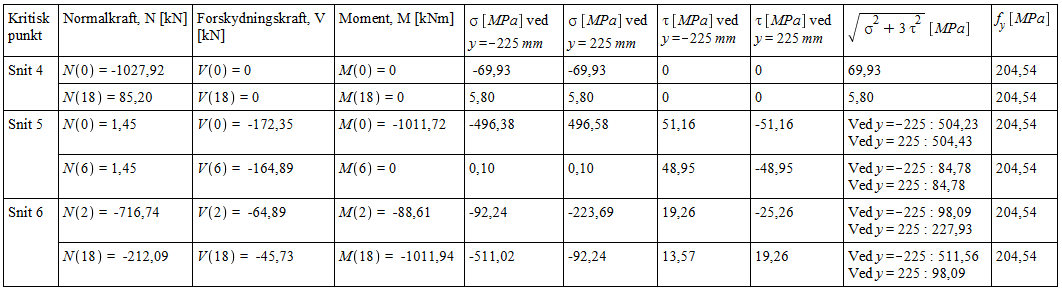
\includegraphics[width=0.8\textwidth]{billeder/tabelspanding.png}
 	\caption{Resultater af spændingstilstand}
 	\label{fig:tabelspanding}
 \end{figure}

Det ses i Tabel \ref{fig:tabelspanding} at spændingen i flere tilfælde overskrider den regningsmsæssige flydespænding. Derfor vil stålrammen opleve brud, og i værste tilfælde knække sammen, som det kendes fra ståls arbejdskurve.
\newline 
\newline
For at konstruktionen ikke skal bryde sammen, skal der foretages en række ændringer.
\newline \indent{     }  Der er indsat tre stålrammer i tilbygningen. Ved at indsætte en eller to stålrammer mere, vil lasterne foredeles ud over disse, og dermed vil hver enkelt stålramme i mindre grad belastes. Dermed vil spændingerne i sidste ende mindskes. 
\newline \indent{     }  Der er valgt en ståltype S235, som kan ændres til en højere styrkeklasse, for eksempel S275 eller S355. Ved at vælge en højere styrkeklasse, øges flydespændingen dermed. En større flydespænding betyder, at stålen kan klare en større spænding. Ved for eksempel kan ændre ståltypen til S355 ændres flydespændingen til $f_y = \frac{345 MPa}{1,\!1} = 313,\!64 MPa$. 
\newline \indent{     }  Til sidst kan der vælges en anden stålprofil. Dette vil ændre henholdsvis højden, bredde, inertimomentet, densiteten, tværsnitsarealet, mm på stålprofilen. Dette vil give anledning til en mindre last, hvis stålprofilen mindskes, og dermed en mindre spænding. 